\documentclass[11pt, oneside]{article}   	% use "amsart" instead of "article" for AMSLaTeX format
\usepackage{geometry}                		% See geometry.pdf to learn the layout options. There are lots.
\geometry{letterpaper}                   		% ... or a4paper or a5paper or ... 
%\geometry{landscape}                		% Activate for for rotated page geometry
%\usepackage[parfill]{parskip}    		% Activate to begin paragraphs with an empty line rather than an indent
\usepackage{graphicx}				% Use pdf, png, jpg, or eps� with pdflatex; use eps in DVI mode
								% TeX will automatically convert eps --> pdf in pdflatex		
\usepackage{amssymb}
\usepackage{amsmath}
\usepackage{parskip}
\usepackage{color}
\usepackage{hyperref}

\title{Properties of complex numbers}
%\author{The Author}
%\section{}
%\subsection*{}
\date{}							% Activate to display a given date or no date

\graphicspath{{/Users/telliott_admin/Dropbox/Tex/png/}}
% \begin{center} 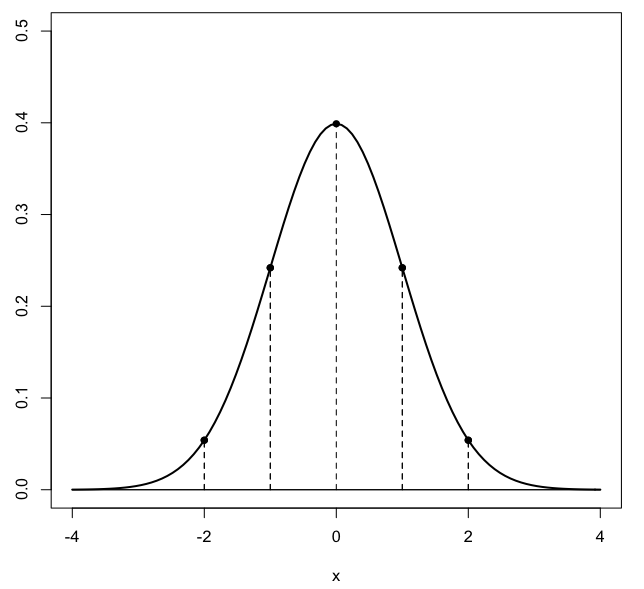
\includegraphics [scale=0.4] {gauss3.png} \end{center}
\begin{document}
\maketitle
\Large
You probably know that complex numbers $z \in \mathbb{C}$ arise in the context of finding solutions polynomials, for example, this equation:
\[ x^2 + 1 = 0 \]
which has no solution among the real numbers.  

It is easy to see this since $x^2$ is always $\ge 0$ for all $x \in \mathbb{R}$, so adding $1$ to $x^2$ cannot bring the sum back to zero.  

Visualizing the same function geometrically, this is the simple parabola $y=x^2$ shifted up, moving its vertex from $(0,0)$ to $(0,1)$.  A plot the function shows that it never crosses the $x$-axis. 

Now, define $i = \sqrt{-1}$, so that $i^2 = -1$, which gives $\pm i$ as the solutions to the above equation.  

Having $i$ available, any square root like $\sqrt{-a}$, where $a$ is a positive real number, can be factored as $\sqrt{a} \ \sqrt{-1} = i \sqrt{a}$.

However, note that the reverse is not necessarily true.  Consider
\[ i^2 = \sqrt{-1} \cdot \sqrt{-1} \stackrel{?}{=} \sqrt{(-1)\cdot (-1)} = \sqrt{1} = 1 \ne -1 \]
The equality with a question mark is \emph{not} valid, which explains why this "proof" is erroneous.

We consider complex numbers $z$ as combinations like $z = a + ib$ where $a$ and $b$ are both real numbers and $b$ is called the imaginary part of the complex number $z$.

In the example above, it is not true that
\[ \sqrt{a} \cdot \sqrt{b} = \sqrt{ab} \]
when both terms are purely imaginary numbers.

Some useful identities involving $i$ include
\[ i^2 = -1 \]
\[ i = -\frac{1}{i} \]
\[  -i = \frac{1}{i} \]

For much of what is done with complex numbers the fact that $i$ equals $\sqrt{-1}$ is not important.

Instead, we simply have ordered pairs of real numbers $(a,b)$ and the $i$ notation is a bookkeeping device, a marker to remind us that when we multiply
\[ (a + ib) (c + id) \]
the result of multiplying $ib \cdot id$ is a real number with the sign flipped, while a real number $a$ times an imaginary number $id$ is equal to $iad$.
\[ (a + ib) (c + id) = ac -bd + i(ad + bc) \]

In other words, a complex number is simply an \emph{ordered pair} such as $(a,b)$.  

Note that if we consider two complex numbers $z_1 = a + ib$ and $z_2 = c + id$, then 
\[ z_1 = z_2 \iff a = c \text{ and } b = d \]
Equality means that both the real and the imaginary parts are equal.

Another way to keep track of the same information is in matrix form, namely:
\[
a + ib = (a,b) =
\begin{bmatrix}
a & -b \\
b &  \ \ a
\end{bmatrix}
\]
Such matrices can be added and multiplied in the normal way and give the desired results for complex numbers.  Thus:
\[
\begin{bmatrix}
a & -b \\
b &  \ \ a
\end{bmatrix} \times
\begin{bmatrix}
c & -d \\
d &  \ \ c
\end{bmatrix} =
\begin{bmatrix}
ac + bd & -ad - bc \\
ad + bc &  \ \ ac + bd
\end{bmatrix} 
=
\begin{bmatrix}
 e & -f \\
f &  \ \ e
\end{bmatrix}
\]
Yet another way to think about complex numbers is to use the complex plane (the Argand plane), where points are plotted with the real part along the horizontal axis and the imaginary part along the vertical axis.

The distance of the point from the origin is equal to $r$, and $\theta$ is the angle the ray makes with the positive $x$-axis in a CCW direction.  
\begin{center} 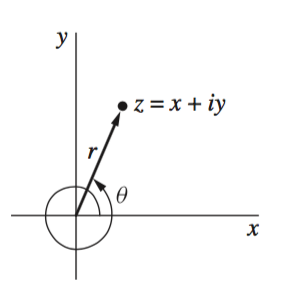
\includegraphics [scale=0.6] {x+iy.png} \end{center}
Switching notation to $x$ and $y$, for the complex number
\[ z = x + iy \]
we have
\[ x = r \cos \theta \]
\[ y = r \sin \theta \]
\[ x + iy = r \cos \theta + ir \sin \theta\]
\[ = r(\cos \theta + i \sin \theta) \]
\[ = re^{i\theta} \]
where the last part makes use of Euler's famous equation.  $r$ is called the \textbf{modulus} and $\theta$ is called the \textbf{argument} or \textbf{phase}.

Notice that in the figure above the argument $\theta$ is actually $\theta + 2 \pi$.  All multiples $2k \pi$ for $k \in 0,1,2 \dots$ are valid.

Calculations may be easier in one form than another.  Addition is simpler with $a + ib$ (the Cartesian format), while multiplication is better with the polar format.  Matrices are fine for both addition and multiplication.
 
Here is multiplication in polar coordinates
\[ r e^{i\theta} \ \rho e^{i\phi} = r\rho e^{i (\theta + \phi)} \]
and 
\[ (r e^{i\theta})^2 = r^2 e^{i2\theta} \]

Multiplication of $z_1 = r e^{i\theta}$ by $z_2 = \rho e^{i\phi}$ stretches $r$ (the length of $z_1$) by the factor $\rho$ (the length of $z_2$), and rotates $z_1$ by adding a phase shift of $\phi$ to the original angle $\theta$.
\subsection*{complex conjugate}
If
\[ z = x + iy \]
then the complex conjugate of $z$ is
\[ z* = x - iy \]

The complex conjugate of $z$ is written as $z*$ or $\bar{z}$.

The \emph{length} of $z$ squared is
\[ zz* = (x + iy) (x - iy) \]
\[ = x^2 + y^2 \]
\[ = r^2 \cos^2 \theta + r^2 \sin^2 \theta \]
\[ = r^2   \]
Again, $r$ is the length of the ray from the origin to $z$ as plotted in the complex plane.
\[ r = \sqrt{zz*} \]
The point corresponding to $z*$ in the complex plane has the same overall length and the same $x$-component as $z$, but the sign change on $y$ means that it is reflected across the $x$-axis.  In polar coordinates, if $z = re^{i \theta}$ then $z* = re^{i (- \theta)} = re^{-i\theta}$.  So
\[ zz* = re^{i \theta} \ re^{i - \theta} = r^2 e^0 = r^2 \]
Alternatively
\[ (x + iy)(x - iy) = x^2 - ixy + ixy -i^2y^2 \]
\[ = x^2 + y^2 \]
The value of $z$ multiplied by its complex conjugate $z*$ is equal to the square of the length $r$.  Multiplication by $z*$ makes the product entirely real.  

If we consider addition rather than multiplication of the complex conjugate we observe that it also gives an entirely real result:
\[ z + z* = x + iy + x - iy = 2x \]
while subtraction gives an entirely imaginary result:
\[ z - z* = x + iy - x + iy = i2y \]

Using the complex conjugate makes it easy to deal with the inverse function:
\[ \frac{1}{z} = \frac{z*}{zz*} = \frac{a - ib}{a^2 + b^2} \]
or in polar notation:
\[  \frac{1}{z} =  \frac{r e^{-i \theta}}{r^2} = \frac{1}{r} \ e^{-i \theta} \]

Let's think about what it means to take the inverse for different $z$.  In every case, the point is reflected across the $x$-axis (the ray has an angle $- \theta$ with the $x$-axis).  

There is no change in length for $r=1$.  But if say 
\[ z = 1 + i = (1,1) = \sqrt{2} \ e^{i \ \pi/4} \]
then the new point has $r = \frac{1}{\sqrt{2}}$ and it is at
\[ \frac{1}{z} = \frac{1}{\sqrt{2}} e^{-i \ \pi/4} = (\frac{1}{2},- \frac{1}{2}) = \frac{1}{2} - i \frac{1}{2}\]

Another result (that we won't prove right now) is that if we have an expression involving several complex numbers:
\[ w = f(z_1, z_2 \dots) \]
we can obtain the complex conjugate of the whole thing by substituting the complex conjugate of each component:
\[ w* = f(z_1*, z_2* \dots) \]

\subsection*{complex functions:  roots}

Consider the value $\sqrt{z}$.  Now, for the modulus part, $\sqrt{r} \cdot \sqrt{r}$ is obviously equal to $r$, and what we need to do for the argument is to find an angle that is one-half of the original one, which leads us to
\[ \sqrt{z} = \sqrt{re^{i\theta}} = \sqrt{r} \ e^{i \theta/2} \]

However, recall from trigonometry (and what we said above) that $\theta + 2k \pi$ is the same angle as $\theta$, for integer $k$.

The same thing is true here.  It is allowed that $\theta = (2k \pi + \theta)$ for $k \in \{ 0, \pm 1, \pm 2 \dots \}$, since it's the same point in the plane.

This means that a second solution to the square root problem is
\[ \sqrt{re^{i\theta}} = \sqrt{r} \ e^{i (\pi + \theta/2)} \]
because, again, $\sqrt{r} \cdot \sqrt{r} = r$ and
\[ \ e^{i (\pi + \theta/2)} \cdot \ e^{i (\pi + \theta/2)} = e^{i (2\pi + \theta)} = e^{i\theta} \]

For the square root, there is only one additional distinct solution, since one-half of $4 \pi + \theta = 2 \pi + \theta/2$ which is no different than $\theta/2$, but the cube root has 3 solutions and in general the $n^{th}$ root has $n$ solutions.

Consider points on the unit circle with $r=1$ (so $\sqrt{r} = r$) and suppose
\[ \theta = \pi/2 \]
so
\[ z = e^{i \pi/2} \]
Points with $\theta = \pi/2$ lie on the imaginary axis (there is no real component).  This point is one unit from the origin so it is the point $(0 + i) = i$.  Thus
\[ e^{i \pi/2} = i \]

$\sqrt{e^{i \pi/2}} = \sqrt{i}$ has two possible values.  One is
\[ \sqrt{e^{i\pi/2}}  = (e^{i\pi/2})^{1/2} = e^{i\pi/4} \]
Let's just check.  The point is at a distance $1$ from the origin and angle $\theta = \pi/4$.  We go equal distances along the real and imaginary axes:
\[ x = \cos \theta = \frac{1}{\sqrt{2}} \]
\[ y = \sin \theta = \frac{1}{\sqrt{2}} \]
So we have that the square is:
\[ (\frac{1}{\sqrt{2}} + i \frac{1}{\sqrt{2}} )^2 = \frac{1}{2} - \frac{1}{2} + 2 i \frac{1}{2} \]
\[ = 0 + i = i \]
the second solution is
\[ \sqrt{e^{i\pi/2}}  = e^{i \cdot 5/4 \pi} \]
which can be plotted as
\[ x = \cos \theta = -\frac{1}{\sqrt{2}} \]
\[ y = \sin \theta = -\frac{1}{\sqrt{2}} \]
The square is the same except the first term is $(- 1/\sqrt{2})^2$, so the result is unchanged.  It's a bit counter-intuitive that squaring a number may possibly reduce the phase angle, but you can think of it as modular arithmetic (mod $2 \pi$).

In general, if we're working with the complex number
\[ re^{i\theta} \]
and we want the nth root, the modulus is just
\[ \rho = r^{1/n} \]
And the question always is, what's the angle?
\[ \phi = \frac{\theta + 2k\pi}{n}, \ \ \ k = 0, 1, 2 \dots n-1 \]

Let's say we want the cube roots of $1$.  Obviously, all the roots will have length $1$.  What about the angles?  The starting angle $\theta = 0$, so $\phi = 2k\pi/3$ and 
\[ \phi_ 1= \frac{2 \pi}{3} \]
\[ \phi_2 = \frac{4 \pi}{3} \]
\[ \phi_3 = \frac{6 \pi}{3} = 0 \]
Notice that the first and second roots are complex conjugates because
\[ \phi_1 + \phi_2 = \frac{6\pi}{3} = 2 \pi = 0 \]

Suppose our number is $z = -8i$ and we want the cube roots.  Writing the number in polar coordinates:
\[ z = 8e^{3\pi/2} \]
All of the roots have the same modulus, $2$, since $2^3 = 8$.  The are three roots which differ in their arguments.  Since $\theta = 3 \pi / 2$, these are:
\[ \phi_1 = \frac{\theta}{3} = \frac{\pi}{2} \]
\[ \phi_2 = \frac{\theta + 2\pi}{3} = \frac{\pi}{2} + \frac{2\pi}{3} = \frac{5\pi}{6} \]
\[ \phi_3 = \frac{\theta + 4\pi}{3} = \frac{\pi}{2} + \frac{4\pi}{3} = \frac{7\pi}{6} \]
Notice that the second and third roots are complex conjugates.

\subsection*{Nahin's puzzle}
In one of his books Nahin starts by posing this question:  suppose we are given that 
\[ x + \frac{1}{x} = 1 \]
\emph{Without computing} $x$, find the value of
\[ x^7 + \frac{1}{x^7} \]
Nahin says that if you are the type to just start right in trying to figure this out, then you will like his book.

From its placement in this section, you might just guess the answer.  First of all, no real $x$ solves the equation
\[ x + \frac{1}{x} = 1 \]
as you will see if you use the quadratic formula.  So let's change nomenclature and call it $z$.  (Of course, we were not supposed to \emph{compute} $z$).

We may guess that $z$ is a complex number with length $1$ so that the lengths don't change with powers or roots.  

Then, all that happens is that $\theta$ changes in such a way that 
\[ 7 \theta = \theta = \frac{\theta}{7}  \]

To actually compute $z$, multiply by $z$, rearrange, and solve:
\[ z^2 + 1 = z \]
\[ z^2 - z + 1 = 0 \]
From the quadratic equation:
\[ z = \frac{1 \pm \sqrt{1 - 4}}{2} = \frac{1}{2} \pm i \frac{\sqrt{3}}{2}  \]
The square of the length is
\[ r^2 = zz* \]
\[ = (\frac{1}{2} + i \frac{\sqrt{3}}{2}) (\frac{1}{2} - i \frac{\sqrt{3}}{2})  \]
\[ = \frac{1}{4} + \frac{3}{4} = 1 \]
The angle we seek has tangent equal to $1/\sqrt{3}$.  You may recognize the sine and cosine of $\pi/3$ as the real and imaginary components of $z$.

So if 
\[ z = e^{i \pi/3} = (\frac{1}{2} + i \frac{\sqrt{3}}{2}) \]
\[ \frac{1}{z} = e^{-i \pi/3} = (\frac{1}{2} - i \frac{\sqrt{3}}{2}) \]
then when doing the addition the imaginary parts of $z$ cancel and we have that 
\[ z + \frac{1}{z} = \frac{1}{2} + \frac{1}{2} = 1 \]

The other special attribute of this value for $z$ is that the length is $1$ so all powers of $r$ are $1$.  As for the angle, $\pi/3$ is special in that $7 \times \pi/3 = 2 \pi + \pi/3 = \pi/3$.  Now it's not strictly true that \emph{the} 7th root of $\theta$ is equal to $\theta$ (since there are 7 distinct roots).  But I hope you can see that there is at least one such root.

\subsection*{powers:  de Moivre's formula}
Let $n$ be an integer:
\[ z^n = (re^{i\theta})^n = r^n e^{in\theta} \]
Suppose $r=1$:
\[ z^n = e^{in\theta} = \cos n \theta + i \sin n \theta \]
\[ (\cos \theta + i \sin \theta)^n = \cos n \theta + i \sin n \theta \]
This is de Moivre's formula.

Suppose $n=2$, then
\[ (\cos \theta + i \sin \theta)^2 \]
\[ = \cos^2 \theta - \sin^2 \theta + 2 i \sin \theta \cos \theta \]
equating with the right-hand side of de Moivre's formula:
\[ = \cos 2 \theta + i \sin 2 \theta \]
we find that
\[ \cos 2 \theta = \cos^2 \theta - \sin^2 \theta \]
\[ \sin 2 \theta = 2 \sin \theta \cos \theta \]
We already know these, they are the double angle formulas.

Suppose $n=3$, then
\[ (\cos \theta + i \sin \theta)^3 \]
\[ = \cos^3 \theta - 3 \cos \theta \sin^2 \theta + i (3 \cos^2 \theta \sin \theta - \sin^3 \theta) \]
we find that
\[ \cos 3 \theta =\cos^3 \theta - 3 \cos \theta \sin^2 \theta \]
\[ \sin 3 \theta = 3 \cos^2 \theta \sin \theta - \sin^3 \theta \]
and so on.

We can just check that last one for $\theta = \pi/6$:
\[ \sin 3 \theta = 3 \cos^2 \theta \sin \theta - \sin^3 \theta \]
\[ 1 = 3 (\frac{\sqrt{3}}{2})^2 \ \frac{1}{2} - (\frac{1}{2})^3 \]
Multiply both sides by $2^3$:
\[ 8 = 3 (\sqrt{3})^2 - 1 \]
That looks correct.

\end{document}  